%
%  This document contains chapter 1 of the thesis.
%
\documentclass[cs,msthesis]{usuthesis}

%{{{ Packages
\usepackage{amssymb}           % add ams symbols stuff
\usepackage{graphicx}          % add graphics
\usepackage{subcaption}
\usepackage{url}
\usepackage{flafter}           % Cause floats to appear after
                               % environment.
                               % MDH: This was originally commented out.
%\usepackage{siunitx}           % Provides standard formatting of SI units.
\usepackage{listings}          % Use when including computer code.

% Include TikZ and PGF packages for high-quality graphics, schematics
% and plots. This is optional; at the current time, when run with
% latex to create a .dvi file, the xdvi viewer will produce incorrect
% formatting for the TikZ figures.  If the .dvi file is converted to
% pdf using "dvipdf" the resulting pdf file is correct.  If this
% example is used with  pdflatex, the resulting TikZ figures in the
% output look fine.
\usepackage{tikz}       		% The base tikz+pgf package
\usetikzlibrary{arrows,shapes}	% Optional tikz extensions
\usepackage[american]{circuitikz}	% TikZ-based package for schematic drawings
\usepackage{pgfplots}			% Tikz-based package for making plots
\pgfplotsset{compat=1.6}        % This *might* be necessary for your
                                % version of pgfplots.

\usepackage{hyperref} % Creates hyperlinks within document
\hypersetup{colorlinks=true, linkcolor=blue,
    citecolor=blue,urlcolor=blue} % Use when compiling the digital copy
% \hypersetup{colorlinks=true, linkcolor=black,
% citecolor=black,urlcolor=black} % Use when compiling the printed copy

% The following allows for hyperlinked DOIs to be inserted in the
% manuscript by using \doi{}.
\usepackage{doi}

\usepackage{enumitem} % MDH: Used for more controls over `enumerate`
\usepackage{amsmath} % MDH: For math functions
\usepackage{amsfonts} % MDH: For math fonts

\usepackage{util} % MDH: Contains my custom commands
\usepackage{notations} % MDH: So I don't have to repeat myself so much
\usepackage{hhline}  % MDH: For double lines in tables
\usepackage{tkz-euclide}  % MDH: To make it easier to label points in Tikz
\usepackage{xfrac}  % MDH: Additional fraction commands
\usepackage{makecell}  % MDH: Better controls in tables
\renewcommand\theadalign{bc}
\renewcommand\theadfont{\bfseries}
\renewcommand\theadgape{\Gape[4pt]}
\renewcommand\cellgape{\Gape[4pt]}
\usepackage{pifont}

% To control where figures are output
\usepackage{epstopdf}
\pdfminorversion=7 % Because epstopdf outputs as version 1.7


% Set spacing around figures and tables to triple space
\setlength{\intextsep}{2em} % Vertical space above & below [h] floats
\setlength{\textfloatsep}{2em} % Vertical space below (above) [t] ([b]) floats

% The following is added if you are using the multiple-paper format to
% add references after each chapter:
\usepackage[sectionbib]{chapterbib}

\newcommand{\vicki}[1]{\textcolor{blue}{Vicki: #1}}

% Author and Title Information
\author{Michael D. Hegerhorst}
\title{
    Proxy Voting Coordination Mechanisms:\\
    Determining How Agents should Coordinate in a Continuous Preference Space
}

% The Committee
\majorprof{Vicki Allan, Ph.D.}
\firstreader{John Edwards, Ph.D.}
\secondreader{Shuhan Yuan, Ph.D.}
%\thirdreader{Gottfried Liebniz, Ph.D.}
%\fourthreader{Isaac Newton, Ph.D.}

% Graduate Dean
\graddean{D. Richard Cutler, Ph.D}
\deantitle{Vice Provost of Graduate Studies}

% Degree Information
\degree{Master of Science}
\month{April}
\gradyear{2023}


\begin{document}
    %{{{ Frontmatter
\preliminaries   % set frontmatter style

\maketitle
\makecopyright        % optional

%
%

\begin{abstract}
% A space is needed before the text starts so that the first paragraph
% is indented properly. Max 350 words.

    Illness, injury, and other impediments are common occurrences of every day life.
    Such impediments prevent or deter agents from participating in important parts
    of the voting process, in particular deliberation, bargaining, and the voting
    itself.
    Without participation, the results of the vote may change.
    There is a need to provide a mechanism by which agents are still able to
    participate in such processes to ensure their vote is represented.
    We examine single-vote/single-winner
    % 05/05/2023: \vicki{Explain unified-vote}
    % Replaced with "single vote," since explaining "unified vote" would probably
    % make may abstract too long.
    proxy voting in a one-dimension continuous
    preference space using a combination of $L_p$ aggregation methods.
    As part of this examination, we develop and examine `coordination mechanisms,' by
    which proxies and their constituents are able to find a way to combine their
    preferences in order for constituents to still have their voices heard.
    In exchange, their proxy gains more weight and is able to have a stronger voice in
    deliberations.
    We employ a continuous preference space model and determine the result of a vote
    as a point in the model's space.
    This model allows for more options than the vote only passing or failing by
    allowing the outcome to directly correlate to actions to be taken, such as the
    amount of money to spend.
    Such an ability increases the granularity of the results and allows us to
    better determine how much error is introduced by proxy voting.
    The continuous preference space model also provides a more expressive way of
    casting a vote.
    We show that proxy voting is effective in many scenarios, and that it is
    consistently better than not allowing inactive agents to vote.


\end{abstract}


% Local Variables:
% TeX-master: "newhead"
% End:

% %
%  Time-stamp: "[publicabstract.tex] last modified by Scott Budge (scott) on
%  2011-08-09 (Tuesday, 9 August 2011) at 09:17:43 on goga"
%
%  Info: $Id$   USU
%  Revision: $Rev$
% $LastChangedDate$
% $LastChangedBy$
%

\begin{publicabstract}
% A space is needed before the text starts so that the first paragraph
% is indented properly.

    % TODO: Rewrite

\end{publicabstract}


% Local Variables:
% TeX-master: "newhead"
% End:
 TODO: Update
% %
% Dedication
%

\begin{dedication}
% \begin{center}
    To Danielle, my constant companion and eternal partner.
    
    You are my light and my star, my guiding hope.
    I love you.
\newline
\newline

    And to Miriam, who joined us in our adventure.
    
    May you lift others up and help them to be as brilliant as you.
% \end{center}
% 
% If you intend to have a dedication longer than one line, do not put
% it in a centering environment.  It will look better.
\end{dedication}
  % optional TODO: Update
%    %
% This is an example of an acknowledgements page.  This is optional,
% and can contain anything you want to say.
%
%
%  Time-stamp: "[acknowl.tex] last modified by Scott Budge (scott) on 2011-08-08 (Monday, 8 August 2011) at 15:45:15 on goga"
%
%  Info: $Id$   USU
%  Revision: $Rev$
% $LastChangedDate$
% $LastChangedBy$
%

\begin{acknowledgments} 
I am so happy that my advisor helped me.....
\\
\begin{flushright} 
John Q. Engineer 
\end{flushright}
\end{acknowledgments}

     % optional TODO: Do I want acknowledgements?

\tableofcontents
\listoftables
\listoffigures

% %
% Contains notations used in this paper.
% Mostly used because I hate having to search throughout a paper to figure
% out what a symbol means in a math equation.
%
%! suppress = EscapeAmpersand
\newcommand{\notationheader}[1]{\multicolumn{2}{l}{\textbf{#1}}\\}
\newcommand{\notationdesc}[2]{#1 & #2\\}

\begin{notation}
\setlength{\tabcolsep}{3mm}{
    % TODO: Alphabetize these by symbol
    \begin{tabular}{ll}
        \notationheader{Equations}
        \notationdesc{\agent}{An individual agent}
        \notationdesc{\agents}{The set of all agents}
        \notationdesc{\cost}{Cost}
        \notationdesc{\loss}{Loss}
        \notationdesc{\real}{The set of all real numbers}
        \notationdesc{\system}{A system}
        \notationdesc{\systemspace}{The space within a system operates}
        \notationdesc{\truth}{Truth}
        \notationdesc{\agenttruth}{The truth as estimated by an agent}
        \notationdesc{\systemagents}{The agents of a system}
        \notationdesc{\systemcost}{The cost of a system}
        \notationdesc{\systemloss}{The loss of a system}
        \notationdesc{\systemtruth}{The truth as estimated by a system}
    \end{tabular}
}

% The table as defined above will fill one page. If you need more room to list
% notation you will need to create a second table, and place it below this 
% comment. This new table will appear one a new page.

\end{notation}

  % optional TODO: Update
% %
% This is an example of an acronyms page.  
% Acronyms are laid out in tabular format.
%
%  Time-stamp: "[acronyms.tex] last modified by Scott Budge (scott) on 2011-08-08 (Monday, 8 August 2011) at 15:45:41 on goga"
%
%  Info: $Id$   USU
%  Revision: $Rev$
% $LastChangedDate$
% $LastChangedBy$
%

\begin{acronyms}

% \renewcommand{\arraystretch}{1.5}
% \setlength{\tabcolsep}{3mm}
% {\begin {tabular}{ll}
% BFCS & body-fixed coordinate system\\
% CEF   &composite energy function (related to ILC)\\
% CSOIS &Center for Self-Organizing and Intelligent Systems\\
% CV    &certainty value (related to HIMM)\\
% DOF   &degree of freedom\\
% EKF   &extended Kalman filter\\
% FOG   &fiber optic gyro\\
% FOV &field of view of a camera\\
% GAIC &geometric Akaike information criterion\\
% GMDL &geometric minimum description length criterion\\
% GRO &growth rate operator (related to HIMM)\\
% HIMM &histogram in-motion mapping\\
% HOSA &higher-order spectral analysis (related to Matlab toolbox)\\
% IBO &identifier-based observer (related to PDS)\\
% IIC &identical initial condition (related to ILC)\\
% ILC &iterative learning control\\
% ICS &inertial coordinate system\\
% LAO &linear approximation-based observer (related to PDS)\\
% LQG &linear quadratic Gaussian\\
% LS &least squares\\
% LTV &linear time-varying\\
% NN &neural network\\
% OCS &obstacle cluster strength (related to HIMM)\\
% ODIS &omni-directional inspection system, a robot at the CSOIS center\\
% ODV &omni-directional vehicle\\
% \end {tabular}}

\end{acronyms}
  % optional TODO: Update
%}}}

    %{{{ The main body of the thesis
    \body  % set main body style
    % Chapters
    \chapter{INTRODUCTION}\label{ch:introduction}
    %%%%%%%% This line gets rid of page number on first page of text
    \thispagestyle{empty}
    %%%%%%%%%%%%%
    From determining the best breakfast cereal~\cite{Curtis2021} to electing the next
    president, voting has become an important aspect of modern society.
    However, disease, injury, and other impediments can create difficulties for individuals
    participating in such democratic processes, preventing them from expressing their
    voice and participating in deliberation, as well as decreasing the overall quality of
    the result.
    Proxy voting is a method by which participants are able to have others vote on their
    behalf.
    We examine the ability of proxy voting to decrease the impact of such frustrations.
    We additionally determine strategies by which proxies and their constituents can
    cooperate in order to reduce the change their absence would otherwise cause.
    These strategies include allowing proxies and constituents to aggregate their
    preference into one result, as well as determining how best to aggregate all votes in
    a unified-vote/single-winner/single-dimension continuous space model.

    \section{Background}\label{sec:background}  % TODO: Maybe rename to "preliminaries?"
\textit{Proxy voting} is a group of methods by which individuals who are unable or
uninterested in voting in person can still have their voices heard through the use of
a \textit{proxy}.
Agents are able to delegate another individual to be their proxy.
We call the delegating agent a \textit{delegator} or an \textit{inactive voter}, and
the group of agents that delegate to a proxy its \textit{constituents}.
Proxies are also known as \textit{delegates} or \textit{active voters}.

Upon selecting a proxy, a delegator is no longer able to vote directly.
Instead, their delegate votes on their behalf in one way or another.
In contrast, \textit{direct voting} requires each agent to vote on their own, meaning
each agent must incur the costs of voting or not have their voice heard.
These costs may be tangible, such as needing to pay for gas, or intangible, such as
being required to vote in-person.
In cases where an agent is unable or unwilling to pay these costs, as in times of
injury or illness, proxy voting provides an excellent avenue through which the agent
can still have its voice heard.

Proxy voting is beneficial for the delegates as well.
By working on behalf of their constituents, a proxy has a larger voice in discussions
and deliberations since they are representing more agents.
This allows them to have a larger influence and achieve a greater impact as
topics are debated.

% Multiple ways of proxies voting TODO: Should this go in our model section?
%   - Congress/Relay
%   - Our model/Single vote
% Why use our model?
%   - Pros
%   - Cons









In order to understand the analysis performed in this study, we must first understand
what proxy voting is and how it works.

In a given voting scenario, every individual starts with one vote.
This vote can be called the voter's \textit{weight} or \textit{voting power}, meaning
each agent starts with a weight of one.
The more weight a voter has, the more they can swing the vote in their favor.
\textit{Proxy voting} involves permitting agents to transfer their voting power
from themselves to another agent, known as a \textit{proxy} or a \textit{delegate}.
These transferring agents are also known as \textit{inactive voters},
\textit{delegators} or \textit{delegating agents}, and the proxies can also be called
\textit{active voters}.
Transferring voting power adds to the voting power of the proxy, increasing its
weight by the amount of power transferred to it.
The group of delegators that transfer their power to the same proxy we'll call its
\textit{constituents}.
By delegating a proxy, the transferring agent loses their ability to directly vote,
instead allowing the proxy to vote on their behalf.
In other words, the transferring agent does not vote in an election or other types of
votes, but rather affects the election vicariously through the proxy to which they
transferred their power.
This allows the delegating agent to skip incurring any costs voting without a proxy
may cause.


Proxy voting has a number of advantages over direct voting.
The most obvious advantage is that it permits delegators to reduce the work and costs
required to participate in a vote by choosing a proxy to perform the work of voting
for them.
Naturally, this is extremely useful when the cost of voting is high, such as
when one is ill or fears they may become ill, or when a member's time can be spent
more efficiently without being physically present for a vote such as when attending a
conference or engaging in active research in some location outside {Washington,~D.C}.
Costs such as these are common in voting scenarios, and are further discussed
in~\cite{Gershtein2019}.
Not being required to be present while still being able to participate is, of course,
directly advantageous for members of the House of Representatives, since proxy voting
would allow them to prevent the spread of disease or avoid whatever other emergency
triggered the use of proxy voting.

There are many ways a proxy could cast their vote on behalf of their constituents.
For example, the proxy could talk to its constituents to see what would make each of
them the most happy and determine an option the would best represent the group as a
whole.
Alternatively, the proxy might decide to selfishly enhance its own voice by voting its
own preference with all the weight allocated to it.
\vicki{Calling it selfish seems too strong. The inactive voters are asking a favor.
It seems weird to say, "Please represent me, but alter your vote to be more what I
want."
}
Such an act might have consequences, such as the proxy no longer being allowed to
represent its constituents and so losing its additional weight.
We will call these different techniques `coordination mechanisms.'
Naturally, requiring the proxy to coordinate with its constituents increases the work
of the proxy, but can provide benefits for the systems in terms of accuracy, as well
as in terms for the proxy by allowing them to aggregate more weight and so allow
their voice to be stronger.
We will explore several of these methods and their impacts in our analysis.

Proxy voting allows voters to skip incurring the costs while still having their voice
heard by allowing a proxy to pay the cost once on behalf of all voters who transfer
their power to that proxy.
However, this advantage comes with the disadvantage that the proxies will likely not
vote in the exact same way as their constituents, meaning the delegators' weights may
not be applied exactly how they want.
The proxy could, of course, confer with its constituents in order determine a vote
that would make them all happy.
However, the proxy could also vote selfishly by voting using only their own preference.
How proxies coordinate with their constituents has a large impact on both the welfare
and the accuracy of the system, and so we will examine proxy voting under both
selfish and cooperative scenarios.

Similarly, proxy voting can be beneficial for the proxies.
By serving as a proxy, an agent can potentially swing a vote more in its favor.
Serving as a proxy also allows the agent to have a stronger voice during
deliberation by showing how many other agents agree with it, or at least how many
have similar opinions.

Since a proxy can vote how it wants, a voter would not want to give its voting power to
just any proxy, but rather one that would still be `close enough' to their preference.
Similarly, a proxy would not want to be a delegate for a voter who does not share a
similar preference, since if the proxy were to attempt to cooperate that voter may
vastly change how the proxy can vote.
There is room for strategy in that a voter could delegate to someone further away in
order to bring the results closer to their opinion.\footnote{
    For example, if an agent that leans only slightly left knows the majority was going
    to vote far left in the preference space, the agent could delegate to someone who
    leans towards the right.
    This delegation would go against the agents desires, but would pull the result of
    the vote more towards the agent's true preference, thereby yielding higher
    utility for that agent.
}\vicki{But this isn't really a function of proxy voting. This is just strategic
voting. They could/would do the same thing if they were physically present.}
These questions on strategy in proxy voting are important, but in order to first
determine if proxy voting would even be useful, this study employs a similar technique
as used in~\cite{Cohensius2017}, which has the voters pass their voting power to the
proxy that is closest in the preference space without any other strategic reasoning.

The `goodness' of a system here is measured using two primary metrics: 1) the
\textit{error} of the system, meaning how close the system is to the optimal
solution, and 2) the total system \textit{welfare}.
Welfare is a measure of how good, or bad, a situation or action is for an agent.
For example, an agent not being required to vote in person increases that agent's
welfare since it makes it easier for the agent to vote.
Conversely, if the agent is required to incur all the costs of voting, such as when
using direct voting, the agent's welfare is lower due to the increased work the agent
needs to do.
Total system welfare is the sum of the welfare of all agents in the system.
An excellent system would have high accuracy and high welfare, while a poor system
would have low accuracy and low welfare.
In regard to proxy voting, the excellent system would maximize the use of proxies
without degrading the accuracy of the system, while the poor would require all
proxies to vote directly and still have high error.
\vicki{Carried to extreme, however, everyone would vote remotely. This discounts the
valuable discussion that happens in meetings.}

Proxy voting has been shown to increase system accuracy when compared to only
allowing active/willing agents to vote~\cite{Cohensius2017}.
This follows intuition: if a voter doesn't vote, the system loses information.
By allowing them to still influence the voting game through proxy, some information
is reintroduced into the system.
Naturally, in terms of system accuracy the ideal situation is when all voters
participate and so the system has the most information possible.
However, system welfare can be enhanced on an individual level by allowing agents
who want to be inactive through the use of a proxy to delegate their vote.
When operating under the Congress resolution, system welfare can be enhanced through
proxy voting by allowing ill members to quarantine and ensure the health of other
agents.
As will be discussed in the results section of the thesis,
% \autoref{ch:results},  % TODO: Uncomment for thesis
this additional system welfare comes at the cost of some system accuracy in terms of
the actual preferences of the voters.
This cost comes about because proxies will likely not vote exactly the same as their
constituents due to having different preferences.
\vicki{If this were the real problem, we could just make proxies vote exactly as
their constituents desired. They could just vote for each one individually. {.2, .3,
.33, .5}. To me the problem is that votes change with discussion, so the proxy is
entrusted to make decisions as amendments and new issues are raised.
%
Before going into specific examples, give us the structure for how proxies operate.
%
Aggregation: mean, median, lp aggregation, plurality
%
Voting: continuous space, finite set of options
    (Note, we are assuming even a finite set of options are ordered. This isn't
    always the case, right? If my vote is between Sarah, Joe, and John, there may not
    be a linear ordering that all agree to.
    %
    Proxy: averages votes of constituents. Votes their own preference.
}

This causes information about the delegators' preferences to be lost and the system's
accuracy to suffer.
The loss in accuracy may be acceptable, however, if the system's welfare is sufficiently
improved.
Perhaps more importantly, proxy voting can also increase system accuracy when a
sufficient number of agents are unable to vote in person, since it allows the system
to recover some lost information by allowing agents to delegate their vote to a proxy
with a similar preference.

% TODO: Move to Future Work section once I have one
% In some cases, the proxy is also able to transfer their own vote, as well as the
% rest of
% their delegated weight, to yet another proxy.
% This is known as \textit{liquid democracy}, which has its own challenges and
% advantages.
% Ultimately, the use of liquid democracy is not considered in this study, but since
% proxy
% voting is a subset of the liquid democracy system, it would likely be possible to
% extend the results of this study to liquid democracy as well.  \vicki{This could be
% described in a future work section, but seems to have no purpose here.}

There are many ways to represent the votes, or preferences, of agents in a system.
Once such way is a continuous space model, such as the one used in~\cite{Cohensius2017}.
This model places voters' preferences in a metric space \systemspace, such as
in~\autoref{fig:system-metric-space}.
In this model, two points that are close together in the metric space represent
similar preferences, while two points that are far apart represent very different
preferences.

\begin{figure}[htbp]
    \centering
    % Built using:
% https://tex.stackexchange.com/a/148253/277236
% https://tex.stackexchange.com/a/380491/277236
\begin{tikzpicture}[scale=7.0]
    \draw(-1,0) -- (1,0) ; % Axis
    \foreach \x in {-1, 0, 1} % Numbers and lower lines
    \draw[shift={(\x,0)},color=black] (0pt,2pt) -- (0pt,0pt);
    \foreach \x in {-1, 0, 1} % Numbers and lower lines
    \draw[shift={(\x,0)},color=black] (0pt,0pt) -- (0pt,-2pt) node[below]{$\x$};

    % Labeled points
    \tkzDefPoint((-4/7), 0){agentA}
    \tkzDefPoint((3/4) , 0){agentB}
    \tkzDefPoint((1/12), 0){agentC}
    \tkzLabelPoint[above](agentA){$\truthof{a}$}
    \tkzLabelPoint[above](agentB){$\truthof{b}$}
    \tkzLabelPoint[above](agentC){$\truthof{c}$}

    \foreach \n in {agentA, agentB, agentC}
    \node at (\n)[circle,fill,inner sep=1.75pt]{};
\end{tikzpicture}
    \caption{
        Example of a 1D preference metric space, where \truthof{x} represents the
        preference of agent $x$.
        The x-axis represents some preference space, where the leftmost point is
        the most preference most against some idea and the rightmost point is the most
        preference most in favor of the same idea.
        Importantly, points towards the center of the space are more ambivalent
        \vicki{ambivalent seems too strong. According to the dictionary: it means you
        have contradictory or mixed feelings about it. Couldn't you just like the
        centrist approach?  }  about
        the topic or prefer a more moderate approach than the extremes on either end.
    }
    \label{fig:system-metric-space}
\end{figure}

Votes are aggregated into an output using a \textit{voting mechanisms} or
\textit{voting rules}.
Two common voting mechanisms are the \textit{plurality} and \textit{mean} voting rules.
The mean mechanism inherently works to a continuous space, since it can take all
preferences, multiply them by their weights, and then average them.
Plurality  \vicki{Define first, before adapting.}, on the other hand, needs to be
adapted to operate in a continuous space.
In our implementation, we will treat plurality as if the proxies themselves were
candidates.
This is similar to the framework in~\cite{Bulteau2021} treating each preference as a
proposal.
As such, the plurality mechanism will select the preference of the active voter with
the most weight.
\vicki{This doesn't seem right, as it gives the advantage to proxy voters. On a
continuous space, plurality doesn't really make sense. This makes more sense to me.
If there are three real options (-1, 0, 1), count the number of voters in equal
ranges about these points. Select the option with the most votes.}

Proxy voting may seem like an extremely attractive option for the House of
Representatives, and other organizations, to use.  \vicki{We aren't ready for this
example as we don't know how the proxies deal with a variety of constituent votes.}
However, it is not without its flaws.
As a simple example, consider a vote taking over preference
space $\systemspace = [-1, 1]$ with agent preferences $\truthof{\agent_1} = -1$,
$\truthof{\agent_2} = 0.25$, $\truthof{\agent_3} = 0.5$, $\truthof{\agent_4} = 1$,
$\truthof{\agent_5} = 0.15$.
Under the mean mechanism, which aggregates opinions by simply taking their mean, if
everyone were to vote we would get the actual preference of the
system: $\systemtruth = 0.18$.
However, if $\agent_2$, $\agent_3$, and $\agent_5$ were to become inactive and select
$\agent_4$ as their proxy, the result would be $\systemtruth = 0.6$.
This is visualized in \autoref{fig:voting-example}.
This is an absolute error of 0.42, or 21\% of the entire preference space!
Ideally the output of a system employing proxy voting would be much closer to the
actual preference of the system, but since the center voters do not have a more
central proxy, the system's output is skewed towards the most extreme voters.

\begin{figure}[htbp]
    \centering
    % Built using:
% https://tex.stackexchange.com/a/148253/277236
% https://tex.stackexchange.com/a/380491/277236
\begin{tikzpicture}[scale=7.0]
    \draw(-1,0) -- (1,0) ; % Axis
    \foreach \x in {-1, 0, 1} % Numbers and lower lines
    \draw[shift={(\x,0)},color=black] (0pt,0pt) -- (0pt,-2pt) node[below]{$\x$};

    % Labeled points
    \tkzDefPoint(-1, 0){agent1}
    \tkzDefPoint(0.25, 0){agent2}
    \tkzDefPoint(0.5, 0){agent3}
    \tkzDefPoint(1, 0){agent4}
    \tkzDefPoint(0.15, 0){agent5}
    \tkzLabelPoint[above](agent1){$\truthof{\agent_1}$}
    \tkzLabelPoint[below](agent2){$\truthof{\agent_2}$}
    \tkzLabelPoint[above](agent3){$\truthof{\agent_3}$}
    \tkzLabelPoint[above](agent4){$\truthof{\agent_4}$}
    \tkzLabelPoint[above](agent5){$\truthof{\agent_5}$}

    \foreach \n in {agent1, agent2, agent3, agent4, agent5}
    \node at (\n)[circle,fill,inner sep=1.75pt]{};


    % Actual preference
    \draw[color=blue, line width=0.5mm, dotted]
    (0.18, 0pt) -- (0.18, -3pt);
    \node[color=blue] at (0.18,-4pt) {$\systemtruth_{actual}$};

    % Preference under proxy vote
    \draw[color=orange, line width=0.5mm, dotted]
    (0.6, 0pt) -- (0.6, -3pt);
    \node[color=orange] at (0.6,-4pt) {$\systemtruth_{proxy}$};
\end{tikzpicture}

    \caption{
        An example vote and its results.
        $\textcolor{blue}{\systemtruth_{actual}}$ is the result when everyone votes,
        and $\textcolor{orange}{\systemtruth_{proxy}}$ is when $\agent_2$, $\agent_3$,
        and $\agent_5$ delegate their vote and make $\agent_4$ a super voter.
    }
    \label{fig:voting-example}
\end{figure}

Previous research has also identified problems with proxy voting.
\etal{Kling} and \etal{Gölz} all investigated a weakness in liquid democracy, a
superset to proxy voting, dubbed `super voters'~\cite{Kling2015,Golz2021}, which are
proxies that receive an extremely large amount of power, while others gain very little.
While \etal{Kling} ultimately determined these proxies tend to use their power
wisely, possibly to avoid estranging those voters who delegate their power to the
proxy, there can be situations where super voters can be problematic with one-off
issues.
For example, in the previous situation $\agent_4$ could be considered a super voter.
If they were to change their preference, say after bribery, threat, or even
something benign such as changing their opinion after a debate, the system's output
could change drastically.
While there are methods to help mitigate the effect of super voters, which
\etal{Gölz}~\cite{Golz2021} explore, the amount of error produced by a proxy vote
system, including that of super voters, is precisely what this paper will explore.

    \section{Previous Work}\label{sec:\chptindicator-previous-work}
Proxy voting is a well-discussed topic, and we build off many author's previous work.

Jonas Degrave~\cite{Degrave2014} implemented a simple model to calculate how much
weight a proxy has.
The model even allows for agents to delegate multiple proxies.
He treated proxy delegations as a digraph where nodes are voters and edges represent
delegating proxies, and created two methods to determine the weights of each proxy.
The first method constructs a linear equation for each agent, consisting of the
agent's original weight plus the weight of the agents that delegate to it.
The second employs an adjacency matrix and uses linear algebra to calculate the
solution.
Ultimately, both methods simply sum the total weight allocated to a proxy.
We will employ the first technique, since it allows for a straightforward way to
delegate voting power that would not be confusing to voters.
However, we will not take full advantage of it by disallowing proxies to delegate to
other proxies, as well as only allowing each agent to delegate one proxy.
Such proxy-to-proxy delegation is known as \textit{liquid democracy}, which has its own
challenges and advantages.
Unfortunately, it can have the effect that delegates might not know who wields their
voting power, and so we will focus on enhancing deliberation in
unified-vote/single-winner/single-dimension continuous space scenarios.

Related to weight, Zhang~and~Grossi~\cite{Zhang2022} explore treating weight as a
probability instead of a count, in addition to simply transferring voting power to
the proxy.
In the probability model, inactive agents spread their weight out amongst several
proxies.
This probability represents the odds the agent would delegate their full weight to that
proxy.
The probability model allows Zhang~and~Grossi to probabilistically predict the
outcome of a vote, and use that model to see if agents can correctly identify some
world state.
They assume that any agent is able to delegate to any other agent.
We share this assumption, though we will only focus on transferring voting power
directly instead of treating it as a probability.

Anurita~Mathur~and~Arnab~Bhattacharyya~\cite{Mathur2017} looked at several voting
mechanisms applied on a single-winner election vote and determined a ranking for
these mechanisms.
\textit{Voting mechanisms}, also known as \textit{aggregation mechanisms}, are
algorithms that take the preferences of all active voters and turn them in to the
output of the system.
They apply these mechanisms on a dataset while looking only at datapoints without a
Condorcet winner.
In their work, they say a mechanism `beats' another if it has a larger fraction of
the population prefer its output over the other's output.
They discover that the GT\footnote{
    Presumably meaning `Game Theory.'
}~method~\cite{Rivest2010} beats all others, the Schulze~method~\cite{Schulze2011}
and Minimax voting mechanisms always agree and beat all other mechanisms besides the
GT method, while Borda beats Copeland and Plurality, and Plurality comes in last.
These mechanisms are briefly described in~\autoref{tab:\chptindicator-mathur-voting-mechanisms}.
This study will also look at voting mechanisms and attempt to determine which
mechanism is best suited for proxy voting.
Our work will differ significantly from theirs, however, as we will explore voting
mechanisms used in a continuous voting space instead of a discrete-space.
Additionally, our mechanisms will be different from the ones they employed since
their mechanisms either do not work in a continuous preference space, or do not work
well with proxy voting.

\begin{table}[htbp]
    % increase table row spacing, adjust to taste
    \renewcommand{\arraystretch}{1.3}

    \caption{
        Definitions for the voting mechanisms used by~\cite{Mathur2017}.
        $n$ represents the number of candidates for some vote.
    }
    \label{tab:\chptindicator-mathur-voting-mechanisms}

    \centering
    \begin{tabular}{| r | p{0.80\linewidth} |}
    \hline
    \thead[r]{Voting \\ Mechanism} & \thead[l]{Description}  \\
    \hhline{|=|=|}
    Borda & {
        Agents rank each candidate, 1 to $n$.
        The candidate ranked first receives $n - 1$ points, the candidate in second
        $n - 2$, etc.
        Whichever candidate receives the most points total wins.
    } \\
    \hline
    Copeland & {
        Agents rank candidates 1 up to $n$.
        Agents are able to leave some blank, all of which will be counted as last place.
        After all agents have ranked the candidates, they are compared pairwise.
        If a candidate is more often ranked better than another, it gets one point.
        If they are more often ranked worse, they get 0 points.
        When the number of ranked better vs ranked worse is equal, the candidate
        receives half a point.
        The candidate with the largest score wins.
    } \\
    \hline
    GT & {
        Agents rank each candidate, and a pairwise margin matrix is generated.
        In the matrix, position $(x, y)$ is the number of rankings that prefer $x$ over
        $y$, minus the number of rankings that prefer $y$ over $x$.
        A zero-sum game is defined, and an optimal mixed strategy computed.
        % \vicki{explain the zero sum}
        A zero-sum game is a situation in which for every point gained by one side,
        the other side looses and equal number of points.
        The winner is then chosen randomly using the optimal mixed strategy.
        See~\cite{Rivest2010} for more details.
    } \\
    \hline
    Minimax & {
        Agents rank every candidate from 1 to $n$.
        Candidates are compared pairwise, where candidate $x$ is compared to
        candidate $y$.
        The score of each comparison is the number of votes candidate $y$ receives
        more than candidate $x$.
        Then, the maximum score for each candidate $x$ (meaning, its largest
        pairwise defeat) is determined.
        The candidate with the lowest (or minimum) maximum score is selected as the 
        winner.
    } \\
    \hline
    Plurality & {
        Each agent selects their favorite candidate.
        The candidate with the most votes wins.
    } \\
    \hline
    Schulze & {
        Agents rank candidates, and are allowed to skip rankings, give the same rank
        twice, or not rank a candidate.
        Candidates with the same ranking are said to be equally preferred, and
        unranked candidates are ranked last.
        Then, a weighted directed graph connecting agents is generated.
        An edge going from candidate $A$ to candidate $B$ with a weight of 10 means
        10 more agents prefer $A$ over $B$ than $B$ over $A$.
        Using this graph, multiple paths are generated between candidates.
        The strength of the path is the sum of the weight of each edge in the path,
        and the path with the highest strength from $A$ is compared to the strongest
        path from $B$.
        The same occurs with paths from $A$ to $C$, $B$ to $C$, etc.
        The candidate that has stronger paths to each individual agent than all other
        agents wins.
    } \\
    \hline
\end{tabular}

\end{table}


\etal{Cohensius}~\cite{Cohensius2017} explore the use of proxy voting in a
continuous metric space using two voting mechanisms: mean, median.
They also explore proxy voting in a binary space using majority.
They discovered proxy voting using any of these mechanisms generally produces lower
error than direct voting with active voters alone.
This is not too surprising: reintroducing information lost through inactive voters,
regardless of the method, ought to help the system.
Nevertheless, they were able to show that proxy voting is effective under a number of
symmetrical and asymmetrical preference distributions, while under both random and
strategic participation.
However, the majority of their research focuses on voting with infinite populations.
While this work would certainly be applicable to larger populations, since a
population of sufficient size will begin to behave like an infinite
population\footnote{
    Naturally, $\lim_{x \rightarrow \infty} x = \infty$.
}, we are more interested in more realistic proxy voting in smaller, finite populations.
As such, we will explore the effects of proxy voting on a finite population of this
size, as well as explore other possible voting mechanisms, inside this continuous
metric space.

\etal{Bulteau}~\cite{Bulteau2021}, develop and experiment with a framework for
aggregating preferences in several spaces using $L_p$ mechanisms.
$L_p$ aggregation methods work by minimizing the sum of distances to the power of $p$
($d^{\,p}$, where $d$ is a distance) between a possible solution and the voters'
preferences.
These mechanisms are particularly useful because they allow fine-tuning of the
aggregation method by changing $p$.
Specifically, in single-dimension single-winner continuous models, they employ $L_1$
(median),
$L_2$ (mean), and $L_{\infty}$ (mid-range, meaning the point between the highest and
lowest agent preference).
They additionally treat any possible value in the space as a potential output as the
system.
They provide a number of remarks and observations for each of these mechanisms, which
we will be borrowing.
However, they examine these mechanisms without weighted votes, which we will have.
As such, we will adapt each of the mechanisms to use weighted votes so they can work
with proxies, and examine how they operate in the continuous space.

James Miller~\cite{Miller1969} imagined a governmental system utilizing proxy voting
in 1969 as a more direct form of a representative democracy.\footnote{
    That is to say, Miller envisioned a system where individuals could directly vote
    for an issue, or elect a proxy to vote for them.
    Naturally, any democracy that uses proxy voting is a representative democracy,
    since the proxy is representing the delegator.
    Nevertheless, it can be argued that Miller's proposal could provide a more direct
    democracy since a voter can directly vote for an issue if they so choose.
}
His work focuses on reworking the current House and Senate systems entirely by using a
more directly involved populace, but his ideas can still be relevant under the current
system.
In particular, he introduces the idea we call \textit{expert proxies},
those being individuals who would `vote as [the delegator] would if only
[the delegator] had the time and knowledge to participate directly'~\cite{Miller1969}.
Additionally, Miller states `a representative should be an expert, or at least
competent, in each field [on which they are voting]'~\cite{Miller1969}.
This is true both in the government as well as other situations where decisions are
made by voting.
As such, we consider scenarios where a proxy is dubbed, at least according to its
constituents, an `expert,' and so the constituents will go with its preference
instead of their own.

    \section{Preliminary Setup}\label{sec:preliminary-setup}
\subsection{The Model}\label{subsec:the-model}
An important part of any study is the model it uses to represent the system being
studied.
We employ a model described by \etal{Cohensius} in their 2017
article~\cite{Cohensius2017}.
This model places voters' preferences in a single-dimension continuous
metric~space~\systemspace, such as in~\autoref{fig:system-metric-space}.
In this model, two points that are close together in the metric space represent
similar preferences, while two points that are far apart represent very different
preferences.
This model works best when an upper and lower bound is provided, such as only
allowing agents to vote in the interval $[-1, 1]$.

\begin{figure}[htbp]
    \centering
    % Built using:
% https://tex.stackexchange.com/a/148253/277236
% https://tex.stackexchange.com/a/380491/277236
\begin{tikzpicture}[scale=7.0]
    \draw(-1,0) -- (1,0) ; % Axis
    \foreach \x in {-1, 0, 1} % Numbers and lower lines
    \draw[shift={(\x,0)},color=black] (0pt,2pt) -- (0pt,0pt);
    \foreach \x in {-1, 0, 1} % Numbers and lower lines
    \draw[shift={(\x,0)},color=black] (0pt,0pt) -- (0pt,-2pt) node[below]{$\x$};

    % Labeled points
    \tkzDefPoint((-4/7), 0){agentA}
    \tkzDefPoint((3/4) , 0){agentB}
    \tkzDefPoint((1/12), 0){agentC}
    \tkzLabelPoint[above](agentA){$\truthof{a}$}
    \tkzLabelPoint[above](agentB){$\truthof{b}$}
    \tkzLabelPoint[above](agentC){$\truthof{c}$}

    \foreach \n in {agentA, agentB, agentC}
    \node at (\n)[circle,fill,inner sep=1.75pt]{};
\end{tikzpicture}
    \caption{
        Example of a 1D continuous preference metric space, where \truthof{x} represents
        the preference of agent $x$.
        The x-axis represents some preference space.
        An agent can have a preference anywhere within this space.
        One way to interpret the model is to have the leftmost point be the most
        against some idea and the rightmost point is the most in favor of the same idea.
        Importantly, points towards the center of the space are the most ambivalent,
        neutral, or central on the idea.
    }
    \label{fig:system-metric-space}
\end{figure}

Such a model is extremely flexible and can be interpreted in different ways.
When applied to binary for-or-against voting problems, options can be placed at either
extreme of the interval.
For example, say a group is choosing whether or not to put pineapple on pizza.
Using the interval $[-1, 1]$, we can place `no pineapple' at -1, and `yes pineapple'
at 1.
Agents vote according to their preference: -1 for no pineapple, 1 for pineapple.
So far, everything works the same as with a normal vote.
However, due to the continuous nature of the voting space and that agents can vote
anywhere in the given interval.
Therefore, agents who don't care one way or the other can vote at 0 instead of being
forced to choose an option.
Additionally, those that are only slightly in favor can choose some value in between
0 and 1.
Once the votes are aggregated, the result can be rounded to whichever option is
closest.
The continuous space allows agents to better express themselves according to what
their actual preference is, instead of being forcibly binned into one value or the
other.

Alternatively, if the majority of the options are about the center, it may be a sign
neither option is satisfactory.
Using the pineapple on pizza example, we can reinterpret 0 to mean the agents want
pineapple on the pizza, but perhaps feel the amount proposed is too much.
By making the agents aware of how 0 will be interpreted, they can express their
dissatisfaction by voting at or around 0.
Normally, voting goes through a bargaining and an enforcement
phase~\cite{Fearon1998}, but if a sufficient number of agents vote close to 0, the
group can reopen discussion about the topic and re-bargain before conducting a new vote.
This enhances the cooperation aspect of voting, and creates a fundamental change:
voting is no longer the end of the process, but rather part of it.

Finally, the continuous space model allows for another, very powerful interpretation:
interpreting the votes and result as continuous values.
For example, say Congress is voting on how much to allocate to the defense budget.
Congress can decide to allocate anywhere between \$0 and \$1,000 (naturally, these
values are not realistic and are meant to be representative).
A voter can place their vote anywhere between those values, and the result of the
vote will how much Congress allocates.
Say there are three voters, each with their own preferences, and all voters are
active (no voter delegates their vote).
Agent $a$ prefers \$750, $b$ prefers \$600, and $c$ prefers \$250.
By averaging these preferences, the system would output
$\frac{\$(750 + 600 + 250)}{3 \text{ voters}} = \frac{\$1600}{3 \text{ voters}} =
\$533.33$, which would be the amount allocated to the defence budget.
Being able to vote on continuous problems and yield a continuous output, as well as
working with binary issues, makes the model extremely flexible and allows it to
tackle any number of problems.

We are also able to easily calculate error using a continuous space.
The error can simply be the distance from the result of the system when all agents
are active, and the result under proxy voting.

The flexibility of the continuous model in both the discrete and continuous realms, its
ability to use different voting rules, easy interpretability, and easy error
calculation are the reasons it is employed in this study.
We will focus primarily on the continuous instead of the discrete output of the
model, since observing the continuous output allows for more granularity in the
differences between proxy and non-proxy voting, as well as in the differences between
voting rules.

\subsection{Voting mechanisms}\label{subsec:voting-mechanisms}
This study also makes use of \textit{voting mechanisms} or \textit{voting rules},
which are functions that map a set of preferences in~\systemspace\ to an outcome that
also exists in~\systemspace.
For these, we take inspiration from \etal{Bulteau}'s~\cite{Bulteau2021} work in
aggregating one-dimensional single-winner elections by using their $L_p$ aggregation
methods, as well as mixing in plurality.
$L_p$ aggregation methods work by minimizing the sum of distances to the power of $p$
($d^{\,p}$, where $d$ is a distance) between a possible solution and the voters'
preferences.
Naturally, since~\cite{Bulteau2021} did not use weighted proxies, these methods need
to be adjusted to allow for weight.
With \agentweight\ representing the weight of an agent \agent\ and \systemproxies\ as
the ordered set of active voters, the mechanisms we use are
\begin{enumerate}
    \item {
        \textit{Median ($L_1$)}, defined as
        $\textbf{md}(\systemproxies) =
    \min\left\{
        \agent_i \in \systemproxies \text{ s.t. }
            \weightof{\agent_i} +
            \sum_{\agent_j \in \systemproxies}^{\agent_{i - 1}} \weightof{\agent_j}
        \geq \frac{\systemweight}{2}
\right\}$.
        Essentially, the median is the agent whose additional weight makes the sum of
        weights becomes equal to or greater than half the total weight of the system.
        The sum will occur in the same order as the ordering of voters in
        \systemproxies.
    }
    \item {
        \textit{Mean ($L_2$)}, defined as
        $\mathbf{mn}(\systemproxies) =
    \frac{1}{\systemweight}
    \sum_{\agent_i \in \systemproxies} {\weightof{\agent_i} \cdot \agent_i}$.
        This is a typical weighted average.
    }
    \item {
        \textit{Mid-range ($L_\infty$)}, defined as
        $\mathbf{mr}(\systemproxies) =
    \frac{
        \agent_{\text{lowest}} + \agent_{\text{highest}}
    }
    {2}
% TODO: I'm not so sure this equation is correct. Should it simply be the unweighted version.
%   Consider how mean and median are calculated. They make sense because each agent has a weight of 1. However, unweighted midrange ignores those weights and simple takes the larges and smallest votes. Should the "weighted" version not also ifnore those weights?$, meaning the weighted
        preference of the of the agent with the lowest preference plus the weighted
        preference of the agent with the highest preference, divided by the sum of
        their weights.
    }
\end{enumerate}
Additionally, we will apply unweighted versions of these mechanisms against all active
voters (to simulate if proxy voting was not allowed), and all voters, inactive and
active (to simulate the best case where all agents vote).
These additional calculations serve as baselines to determine how well proxy voting
works in these scenarios.

% TODO: Do I still need to explain them more, since I've shown the equations?
% More details on how each voting mechanism operates will be described in the full thesis.
% % in~\autoref{subsec:voting-mechanisms}.  % TODO: Uncomment for thesis

\subsection{Coordination Mechanisms}\label{subsec:coordination-mechanisms}
There are also several ways an individual proxy can agree to cast its vote own behalf
of its constituents.
Each has different advantages and disadvantages for the proxy, its constituents, and
the system as a whole.
We will examine four of these different `coordination' mechanisms:
\begin{enumerate}
    \item {
        \textit{No preference change - Selfish}.
        The proxy allocates its weight to its own preference.
    }
    \item {
        \textit{No preference change - Cooperative Mean}.
        The proxy allocates its weight to the mean of its and its constituents'
        preferences.
    }
    \item {
        \textit{No preference change - Cooperative Median}.
        The proxy allocates its weight to the median of its and its constituents'
        preferences.
    }
    \item {
        \textit{Preference change - Selfish}.
        The proxy allocates its weight to its own preference, but its preference has
        changed.
        This change may be due to additional deliberation or some other cause.
    }
    \item {
        \textit{Preference change - Consequences}.
        The proxy allocates its weight to its own preference, but its preference has
        changed.
        However, due to this change the proxy is only allowed to apply its own
        weight, leaving its constituents unrepresented.
    }
\end{enumerate}
These mechanisms are used in an attempt to simulate real-world consequences of proxy
voting, as well as identify potential techniques to deter or mitigate a proxy's
ability to swing the system by aggregating a large amount of weight and abusing it.

    \section{Assumptions}\label{sec:assumptions}
In order to conduct this study, we make a number of assumptions.
First, we assume that voting issues are one off, meaning agents vote on only one
topic at a time.
This allows agents to select a proxy that works best for the current topic instead of
selecting the best proxy for all topics.

Additionally, we only consider scenarios where single-vote proxy voting is used, where
the proxy receives the voting power of the delegating voter, increasing their weight,
and proceeds to allocate all their weight towards one vote instead of relaying their
constituents vote.
This type of proxy voting also allows the proxy to update their (and by extension, their
constituents) preferences as new information becomes available.
While single-vote proxy voting gives substantial flexibility to the proxy to operate
on behalf of their constituents, this flexibility requires the delegating voter to
choose a proxy who they trust to vote as close to how they themselves would.
This is a process similar to selecting experts, as described by~\cite{Miller1969}
and~\cite{Mueller1972}.
By using single-vote proxy voting instead of relay-style voting, we hope to exploit
the advantages of proxy voting that the relay-style does not provide.

We also assume that each voter has reasonable knowledge of potential proxies'
opinions, meaning they have a decent idea of the preferences of other proxies.
This will allow them to choose the proxy that has the opinion most similar to their own.
While in reality voters will likely not have perfect knowledge of others' opinions,
it is often not particularly difficult to gauge the opinion of others, especially
those with whom an individual often associates, and so we believe this assumption is
reasonable.

Finally, we assume that there are no factors besides closeness in opinion that affect
the choice of proxy.
This differs from some systems, such as that presently used by the House of
Representatives which includes restrictions such as a proxy can only serve ten
voters~\cite{CERP2020}.
However, we feel removing restrictions such as these leads to a more interesting
discussion, since it allows the use of different voting mechanisms and more extreme
cases.

    \section{Contribution}\label{sec:contribution}
We explore proxy voting in a unified-vote/single-winner single-dimension
continuous space model.
We employ three well-known $L_p$ mechanisms, specifically
\begin{enumerate}
    \item {
        Median ($L_1$)
    }
    \item {
        Mean ($L_2$)
    }
    \item {
        Mid-range ($L_\infty$)
    }
\end{enumerate}
Each of these mechanisms will additionally be applied to direct voting with all
agents and direct voting with only those agents that are present.
This is done to show what the output of the system would be with all information
(direct voting with all agents), as well as the output with minimum information
(direct voting with only those agents that are present).
The error will be the distance between the result and direct voting with all agents.

We additionally apply what we've dubbed `coordination mechanisms,' which are
techniques by which proxies and constituents work together to determine how their
weight will be allocated, meaning how the proxy will vote on their behalf.
The mechanisms we explore are described
in~\autoref{subsec:coordination-mechanisms}.
These mechanisms are used in an attempt to simulate real-world consequences of proxy
voting, as well as identify potential techniques to deter or mitigate a proxy's
ability to swing the system by aggregating a large amount of weight and abusing it by
misallocating it towards a vote the constituents don't prefer.
% 05/05/2023: \vicki{
%   Not clear what the abuse refers to.
%   They got the weight fairly.
%   Is the abuse in threatening to change the preference for all?
%   Not all aggregation methods would permit abuse???
% }
% I've added something to specify "abuse" means "misallocating."
% Some voting mechanisms (which I assume is what is meant by "aggregation methods")
% may not permit abuse, but inactive voters don't participate in the voting
% mechanisms; they vote through the proxy.
% This means the coordination mechanism needs to discourage the proxy from abusing
% (misallocating) its constituents votes.
%
% If "aggregation methods" was supposed to mean "coordination mechanisms," the
% methods that don't permit abuse only apply to when the proxy and its constituents
% are choosing their group preference, but wouldn't help when the proxy actually goes
% to cast the vote. To combat misallocation abuse, we introduce the "with
% consequences" coordination mechanisms.

Whereas voting on a continuous interval is uncommon and finding a real world dataset
using preferences on an interval currently does not seem possible, these investigations
are performed using preferences generated from several statistical distributions.
We use various distributions to allow the gathered data to represent
different distributions of voters in the real world.
These distributions include well-known statistical distributions, such as the uniform
distribution, the Gaussian distribution, as well as a few beta distributions.
The distributions used and their notations are listed
in~\autoref{tab:distributions-used}.

\begin{table}[!htbp]
    % increase table row spacing, adjust to taste
    \renewcommand{\arraystretch}{1.3}

    \caption{
        The distributions to be used to generate preferences.
        Note how each distribution represents a population type.
        These types are representative, and any distribution could potentially
        represent a different population type that shares the same shape as the
        distribution.
        Additionally, any skewed distributions can be inverted to create a
        distribution that is skewed in the other direction (e.g. a distribution
        skewed in favor can be inverted to create a flipped distribution skewed
        against).
    }
    \label{tab:distributions-used}

    \centering
    \begin{tabular}{|r|l|c|l|}
    \hline
    \thead{Distribution} & \thead{Notation} & \thead{Symmetrical?} & \thead{Population Type}
    \\
    \hhline{|=|=|=|=|}
    Uniform & \uniform{-1}{1} & \ding{51} & Evenly spread
    \\
    \hline
    Normal/Gaussian & \gaussian{0}{\sfrac{1}{3}} & \ding{51} & Mostly
    centrist/indifferent
    \\
    \hline
    Beta(0.3, 0.3) & \betadistribution{0.3}{0.3} & \ding{51} & At either extreme
    \\
    \hline
    Beta(50, 50) & \betadistribution{50}{50} & \ding{51} & Strongly
    centrist/indifferent
    \\
    \hline
    Beta(4, 1) & \betadistribution{4}{1} & \ding{55} & Skewed in favor
    \\
    \hline
\end{tabular}
\end{table}

Initial experiments show larger populations behave similarly to those with fewer.
As such, each experiment will have a population of 24.
We chose this number because prior experimentation shows it to be a good balance
between having few enough agents that an agent going inactive can change the
results, while not so few that an agent going inactive is catastrophic.
Since having no delegates or all delegates would not be interesting, we will
experiment with 1 to 22 inactive agents and examine how error correlates with
the number of delegators.
We choose 1 inactive agent as the minimum because the case with 0 agents is not
interesting due to there not being any proxies.
% 05/05/2023: % \vicki{I thought you did consider 0?}
% No, I never have. As we've discussed, having 0 inactive agents is the same as not
% using proxy voting and is not interesting. This plan was specified in the proposal.
% Instead, I was asked to extend my graphs to include 0 (which I did by actually
% running the simulations with 0 inactive agents).
Similarly, we chose 22 as the maximum because the case with 24 agents means there are
not active agents to vote, and the case with 23 simply devolves into the coordination
mechanism replacing the voting mechanism.

For each experiment, agents will randomly select some preference using the current
distribution.
Afterward, one agent
% \vicki{sounds like various numbers of inactive voters are used.
% Can you state that initially?}
% MDH: This is stated in the previous paragraph. I've reworded it slightly to make it
% more clear.
will become inactive and choose the closest active agent to be their proxy.
Following this, the proxies and their constituents will apply a coordination
mechanism, and each voting mechanism will be applied.
The next coordination mechanism will be used, then each voting mechanism will be
applied again.
Once all coordination mechanisms have been used, the number of inactive agents will
increase 22 agents are inactive.
% 05/05/2023: \vicki{Earlier you said 22 is the maximum}
% Whoops, that was a leftover from when I was running up to 23. I've fixed it to be
% correct.
Finally, agents will select a new preference from the next distribution and the
process will begin again.
This will continue until all possible combinations have been used.
% 05/05/2023 \vicki{
%   For each experiment, are preferences and inactive voters re-selected?
%   The way you discuss it, it sounds like the steps are additive.
%   If they aren't there is no need to describe it as a progression.
%   You should also state that each experiment was run 1024 times.
% }
% The preferences are reselected whenever a new preference distribution is used, as
% stated two sentences prior. Since we only want to change one variable at a time
% (similar to not using different RNG seeds), we only change the preferences once all
% combinations have be used. This way, each coordination mechanism and voting
% mechanism is applied to the same preferences with the same proxies and inactive
% voters.
%
% I've specified the number of runs below.
Each combination is run 1024 times to ensure any accuracy in the analysis.

We will show that proxy voting with the right combination of mechanisms generally
yields considerably lower error than active-only voting.
We also show proxy voting is beneficial even when agents' preferences change.
However, proxy voting appears to be least effective on highly-polarized topics.


    % Endmatter
% For BibTeX references: specify a .bib file and a style.
% The style used here is for IEEE transactions formatting:
\references{references/IEEEabrv,references/research}{IEEEtran}

% %
%  Example Appendix pages.
%  Modified to use new usu-thesis-mk2 appendix facilities.
%
%  Time-stamp: "[appendix.tex] last modified by Scott Budge (scott) on
%  2021-06-28 (Monday, 28 June 2021) at 09:03:44 on goga.ece.usu.edu"
%
%  Info: $Id: appendix.tex 1183 2021-06-28 16:49:30Z scott $   USU
%  Revision: $Rev: 1183 $
% $LastChangedDate: 2021-06-28 10:49:30 -0600 (Mon, 28 Jun 2021) $
% $LastChangedBy: scott $
%
%
% For a single appendix, use \makeappendix, and place the 
% body of the appendix after it

%\makeappendix

% < single appendix body here >

% For multiple appendices, use \makeappendices, and create each appendix
% using \appendix{}
% For sub-appendices use \appendixsection{} and \appendixsubsection{}

\makeappendices
\appendix{Voting Distributions}\label{chap:voting-distributions}

\appendixsection{Percent inside Extents}
% TODO: Add description of table
This is placeholder text to ensure
\autoref{tab:distributions-percent-inside-extents} stays in the correct
location. % FIXME

% - Distribution of votes
%     - Uniform
%     - Gaussian
%     - Bimodal about center
%     - Skewed?

\begin{table}[htbp]
    % increase table row spacing, adjust to taste
    \renewcommand{\arraystretch}{1.3}

    \caption{List of distributions used by agents to vote.}
    \label{tab:distributions-percent-inside-extents}

    \centering
    \begin{tabular}{|c|c|c|}
        \hline
        Distribution      & Notation      & Percent inside Extents \\
        \hline
        Uniform           & \uniformdist  & 100\%                  \\
        \hline
        Normal (Gaussian) & \gaussiandist & 99.7\%                 \\
        \hline
        Beta              & \betadist     & 100\%                  \\
        \hline
    \end{tabular}
\end{table}

\appendixsection{Distributions used}
% TODO: Add graphs of distributions used
\begin{table}[htbp]
    % increase table row spacing, adjust to taste
    \renewcommand{\arraystretch}{1.3}

    \caption{List of distributions used by agents to vote.}
    \label{tab:distributions}

    \centering
    \begin{tabular}{|c|c|c|}
    \end{tabular}
\end{table}

\appendixsection{Voting Mechanism P-Values}
\autoref{fig:all-voting-mechanisms-p-values} illustrates the p-values for all voting
mechanisms, given the alternative is one population is lesser than the other.
An arrow pointing to another voting mechanism indicates the `from' mechanism beats
the `to' mechanism.

\begin{figure}[!t]
    \centering
    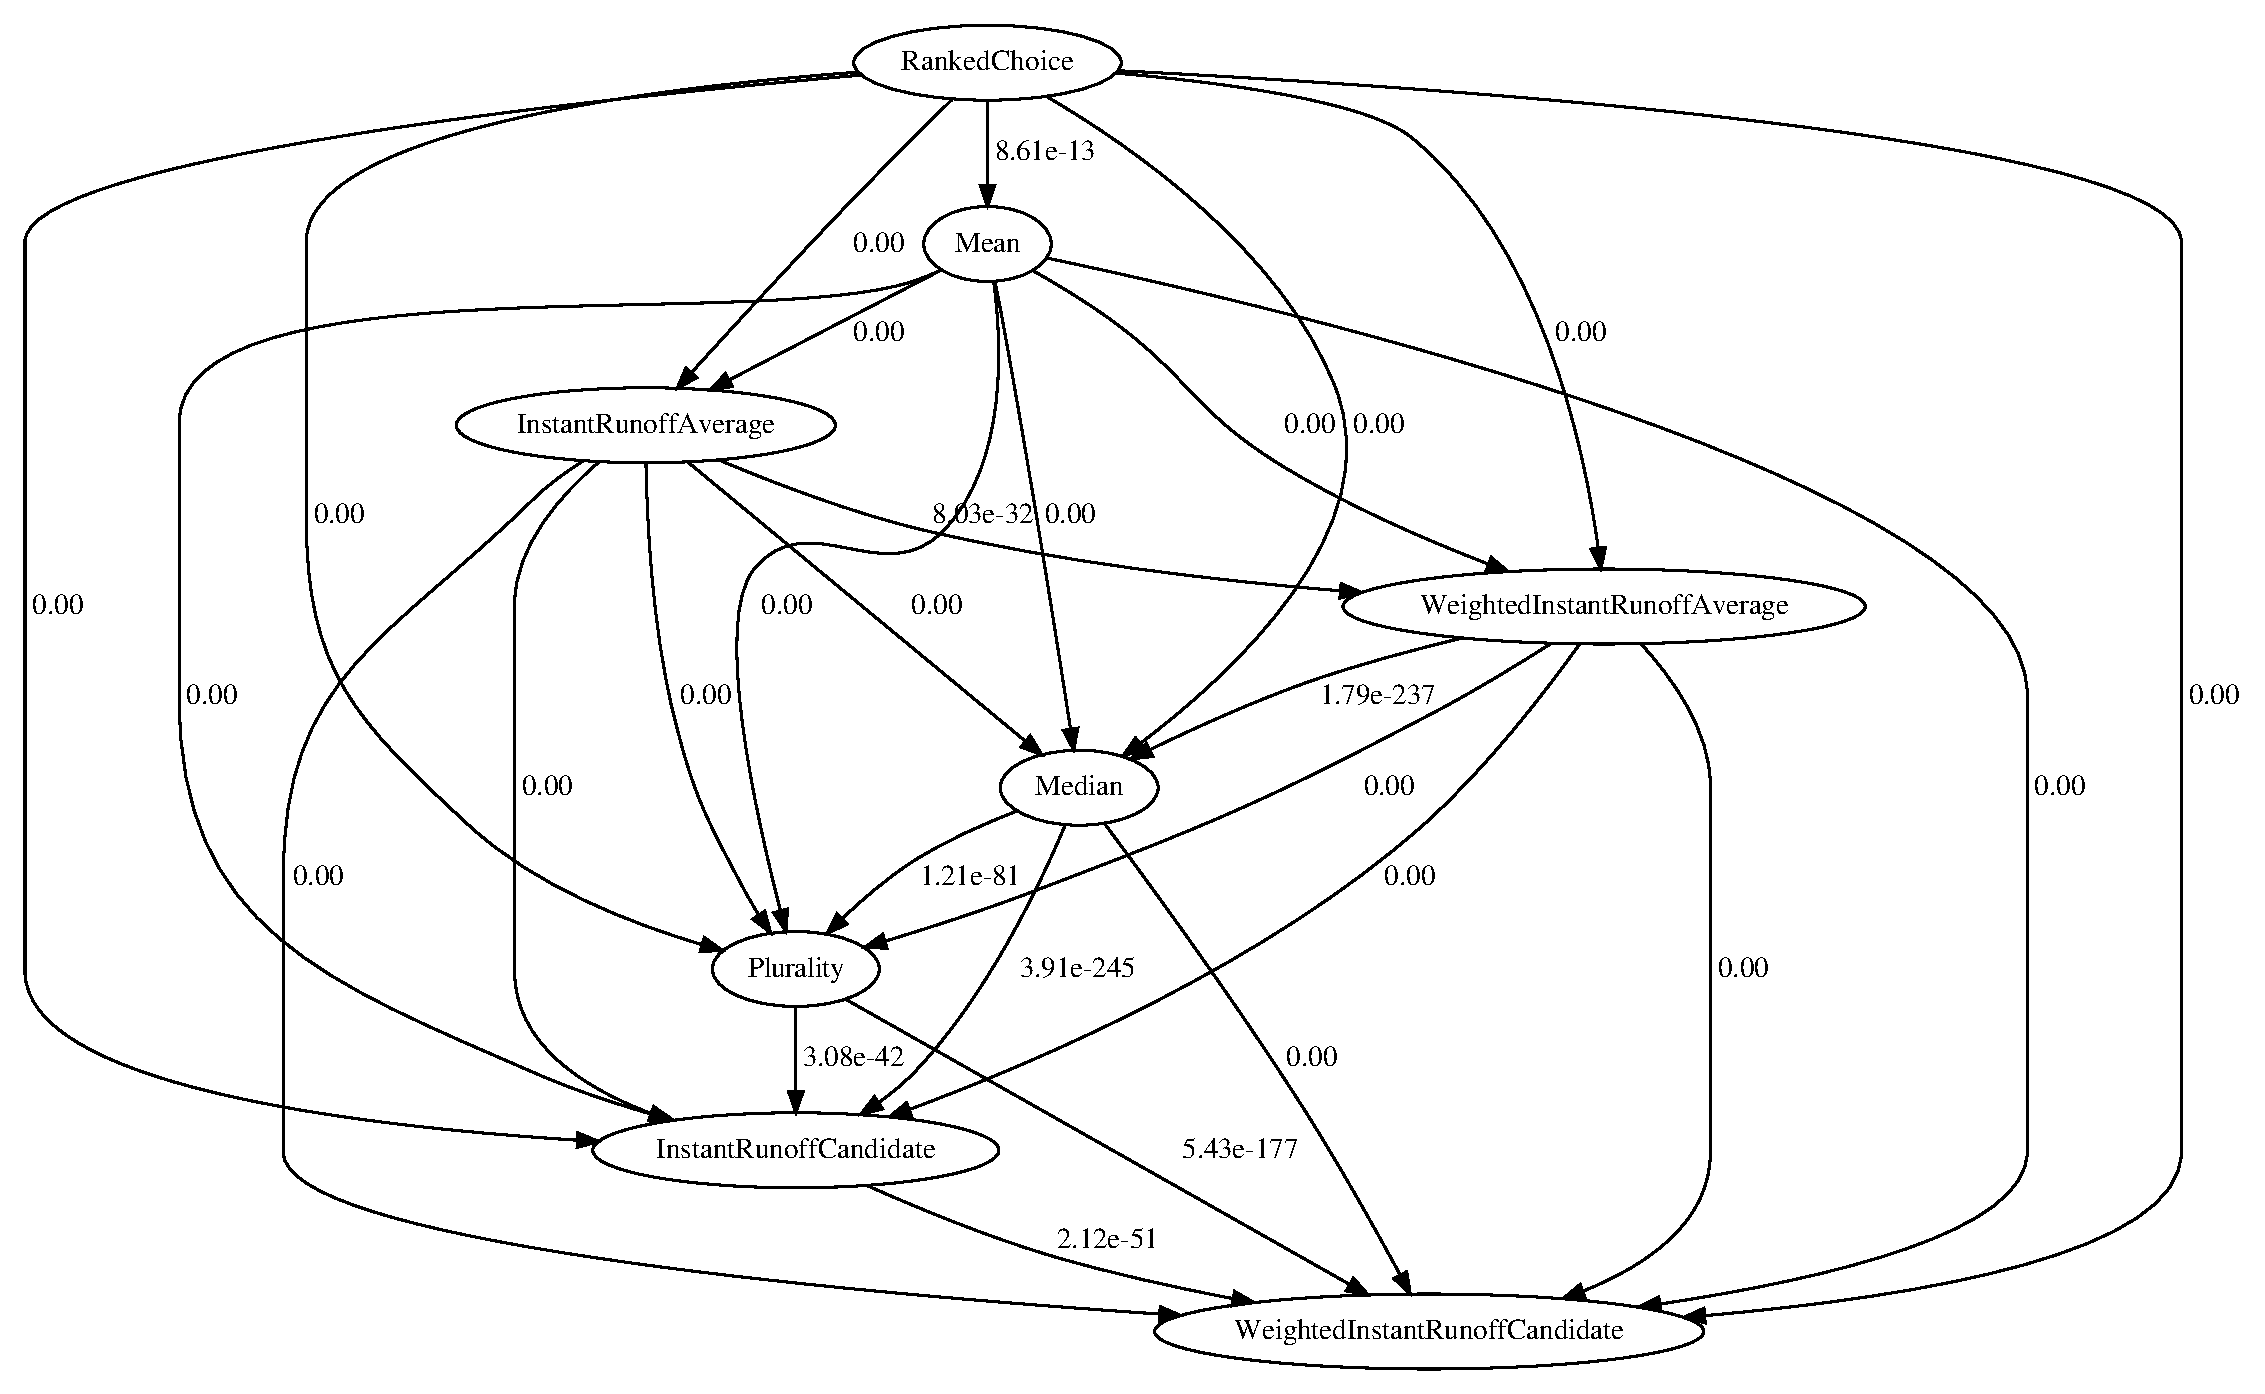
\includegraphics[
        angle=90,
        width=\textwidth,
        height=\dimexpr
        \textheight - 4 % Could also be .9\textheight
        \baselineskip,
        keepaspectratio]
    {./content/figures/voting_mechanisms/all-voting-mechanisms-p-values.gv}
    \caption{The p-values for all voting mechanisms, given the alternative is one
    population is lesser than the other.
    An arrow pointing to another voting mechanism indicates the `from' mechanism beats
    the `to' mechanism.}
    \label{fig:all-voting-mechanisms-p-values}
\end{figure}


\appendixsection{Distributions of Variables}
The distribution of variables for each voting mechanism is displayed as a
KDE graph in the figures of this section.

\begin{figure}[!t]
    \centering
    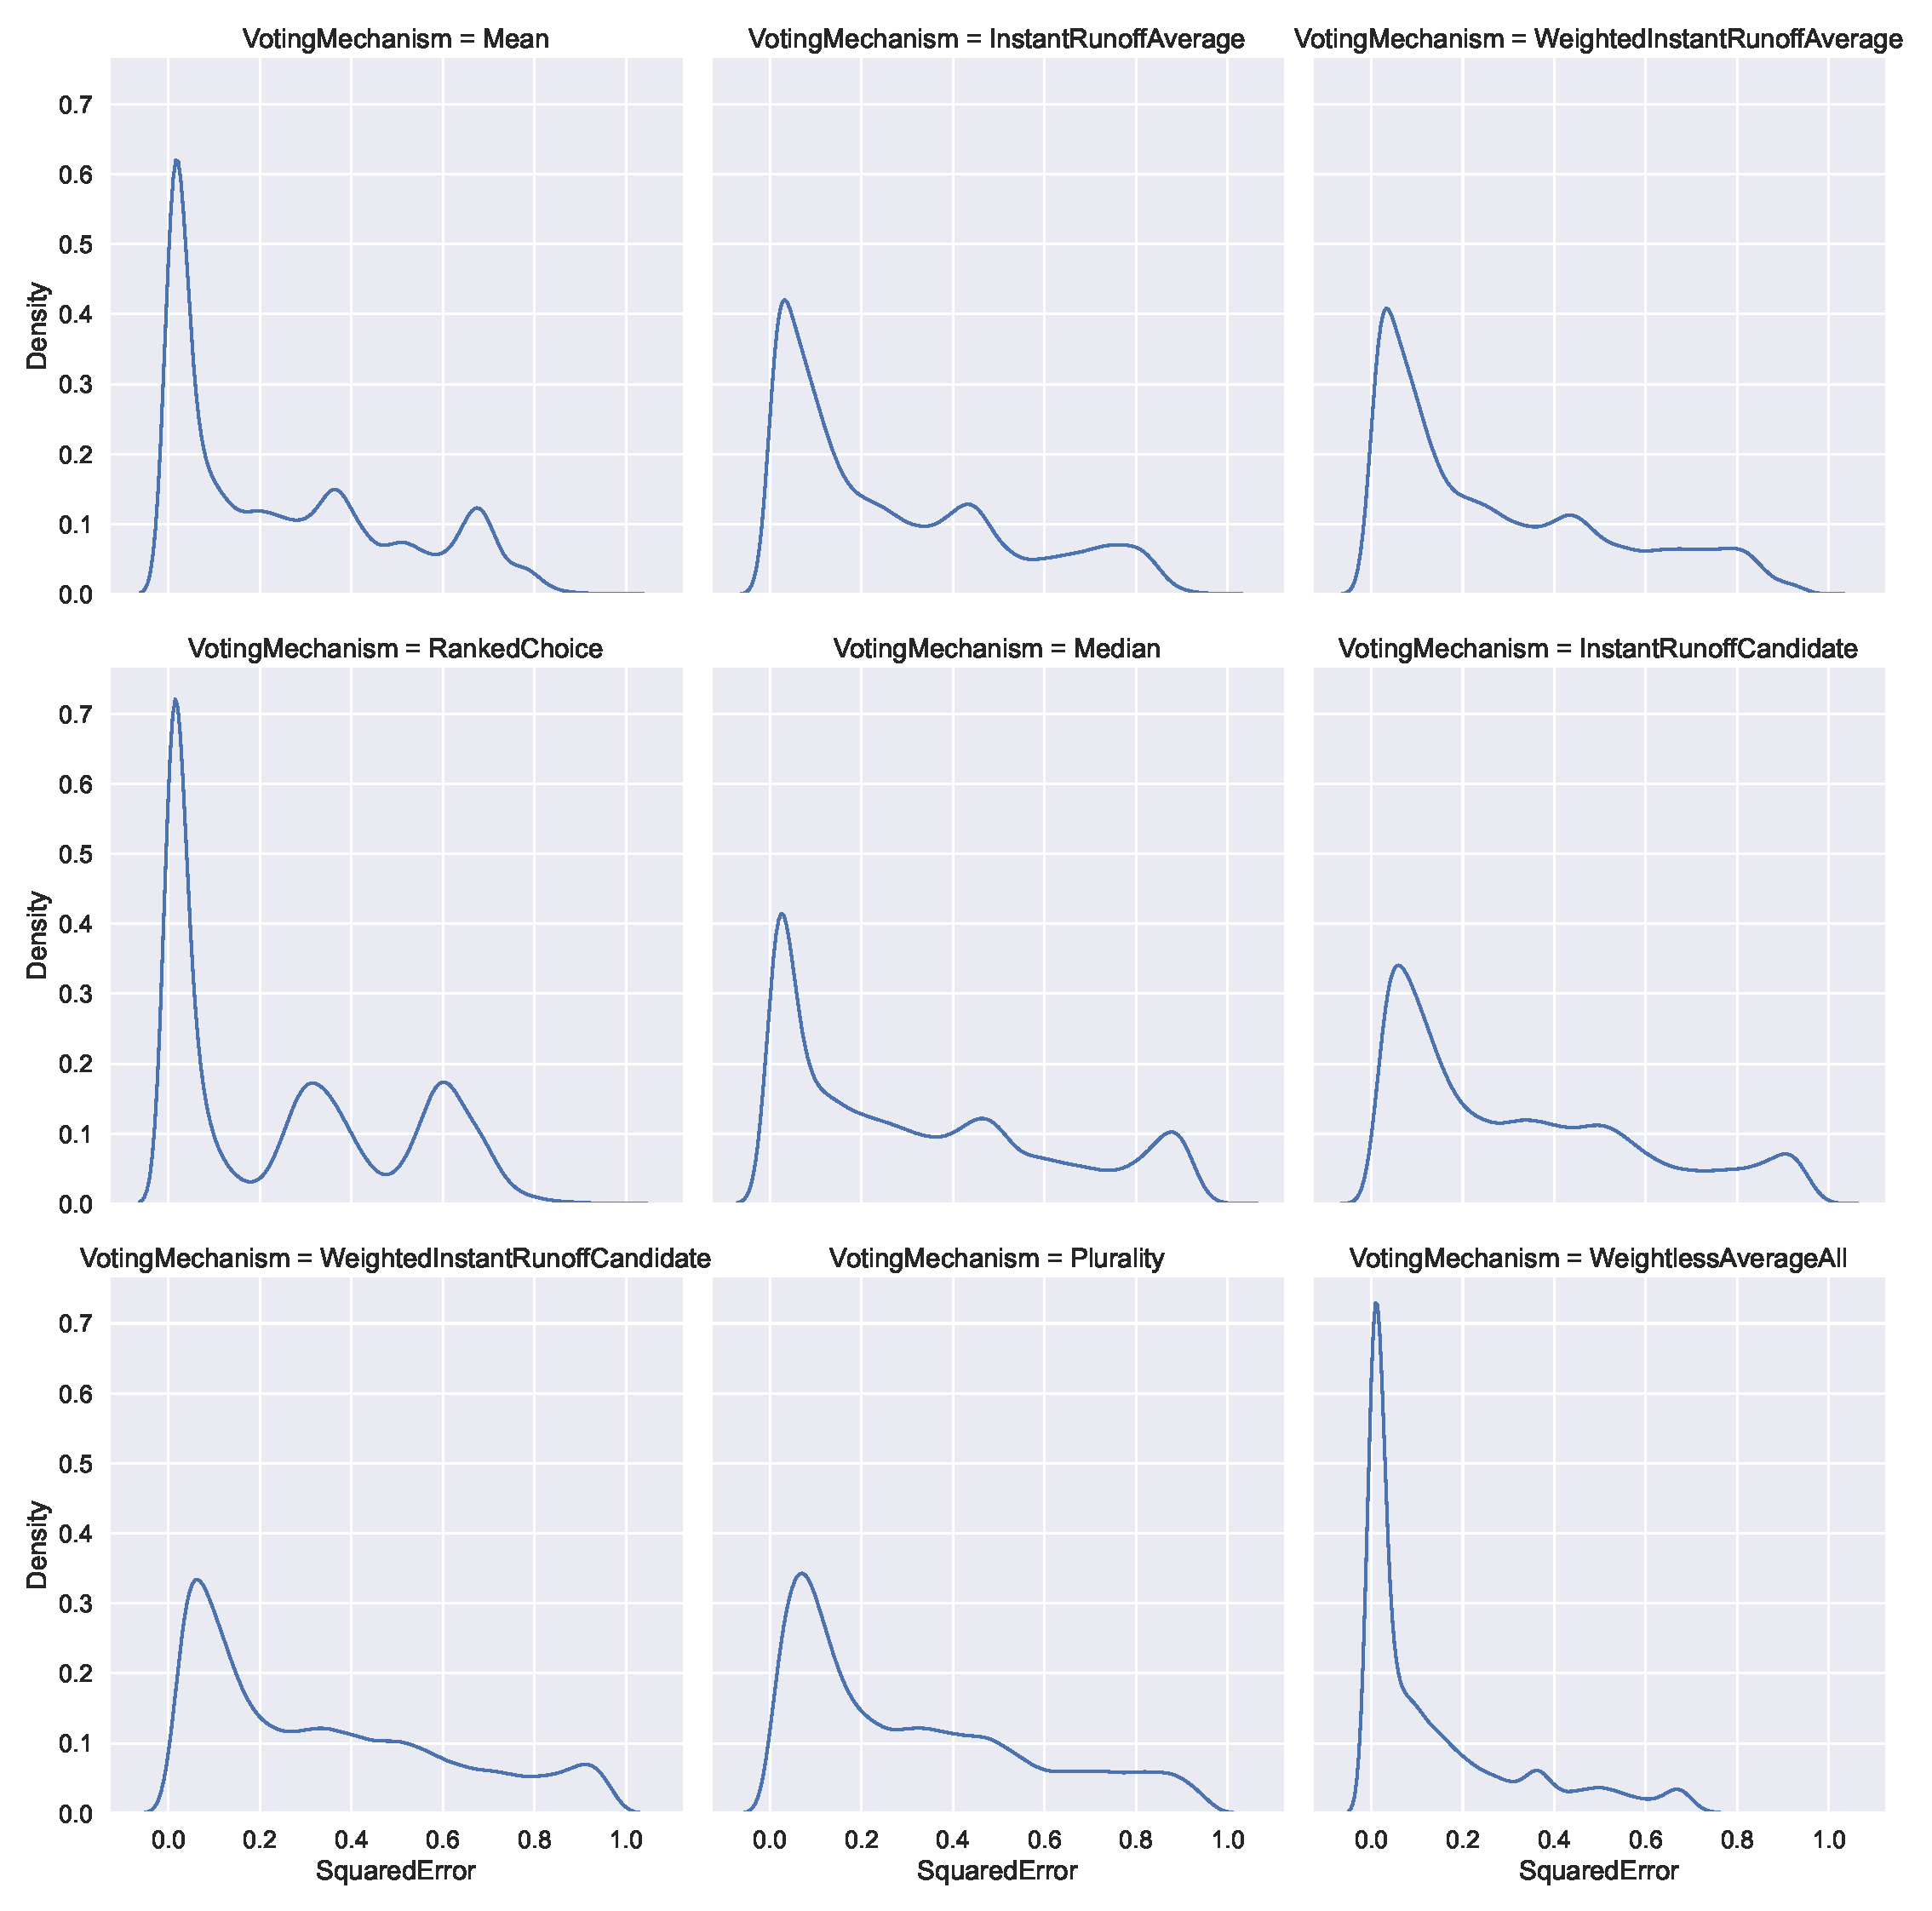
\includegraphics[
        width=\textwidth,
        height=\dimexpr
        \textheight - 2 % Could also be .9\textheight
        \baselineskip,
        keepaspectratio]
    {./content/figures/voting_mechanisms/voting_mechanisms_error_distribution}
    \caption{The distribution of squared error by voting mechanism.}
    \label{fig:voting_mechanisms_error_distribution}
\end{figure}

\begin{figure}[!t]
    \centering
    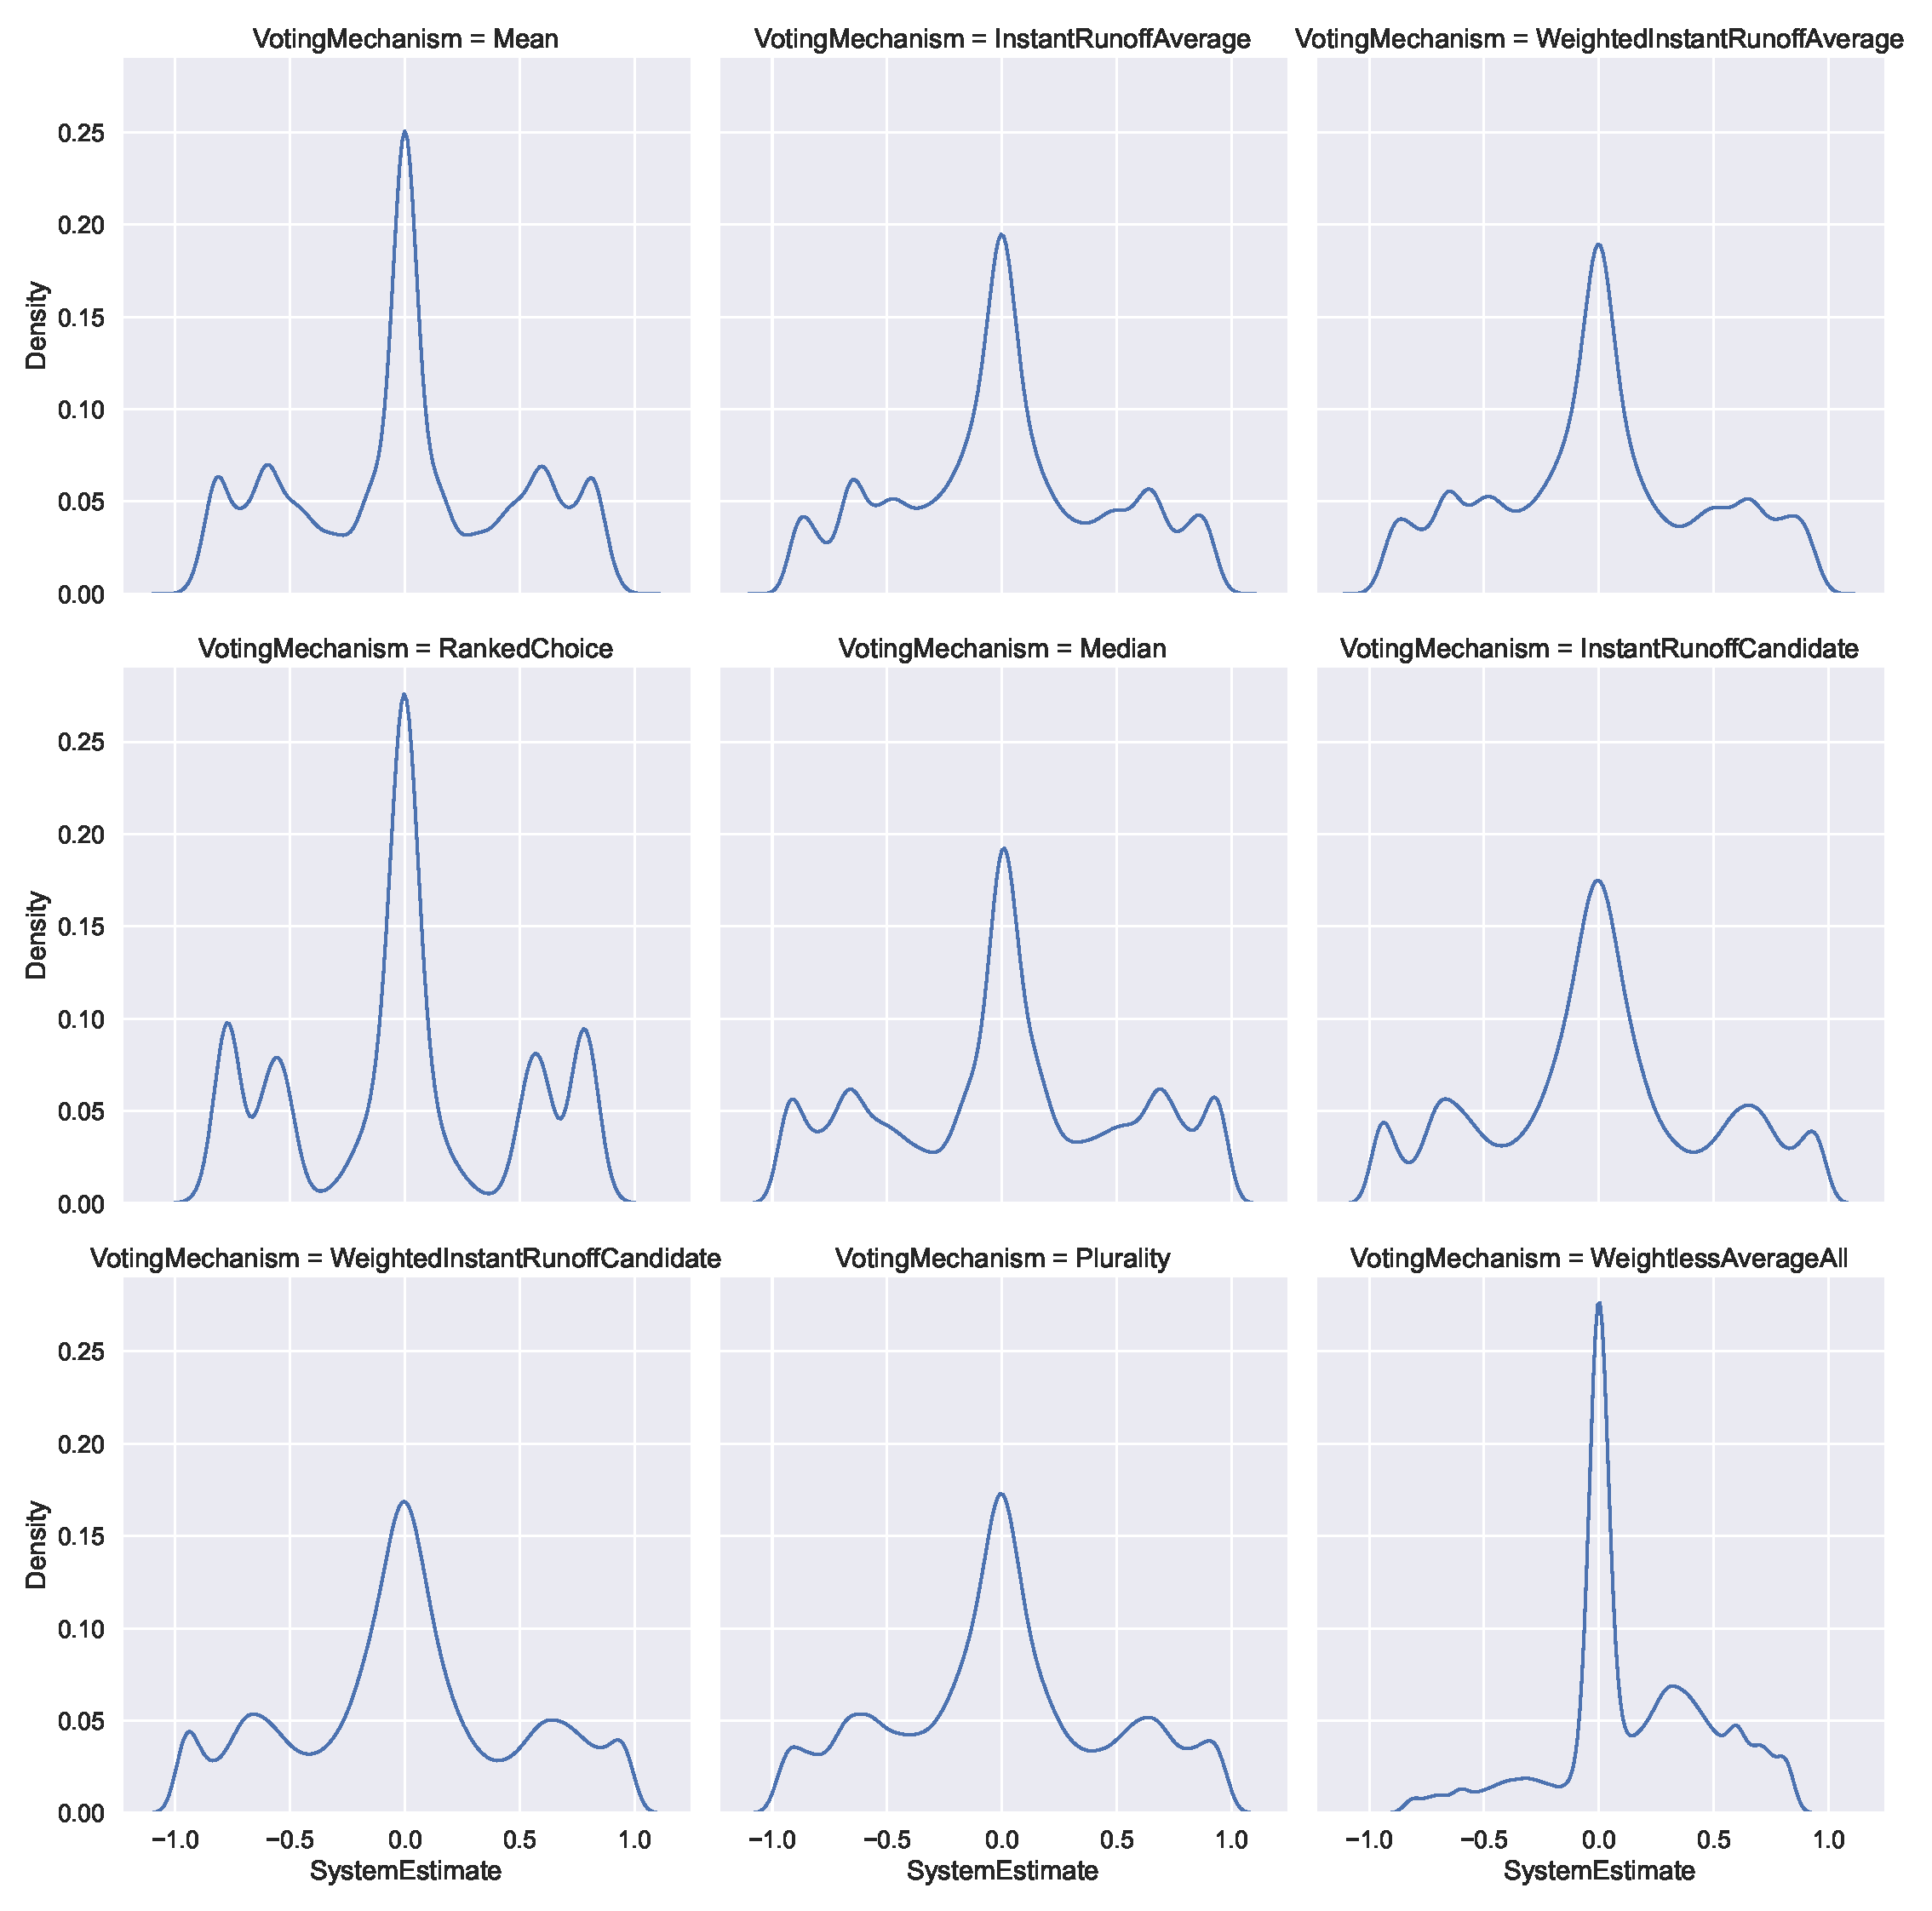
\includegraphics[
        width=\textwidth,
        height=\dimexpr
        \textheight - 2 % Could also be .9\textheight
        \baselineskip,
        keepaspectratio]
    {./content/figures/voting_mechanisms/voting_mechanisms_estimate_distribution}
    \caption{The distribution of system estimate by voting mechanism.}
    \label{fig:voting_mechanisms_estimate_distribution}
\end{figure}

\appendix{Visualizations}\label{chap:visualizations}
\begin{figure}[htbp]
    \centering
    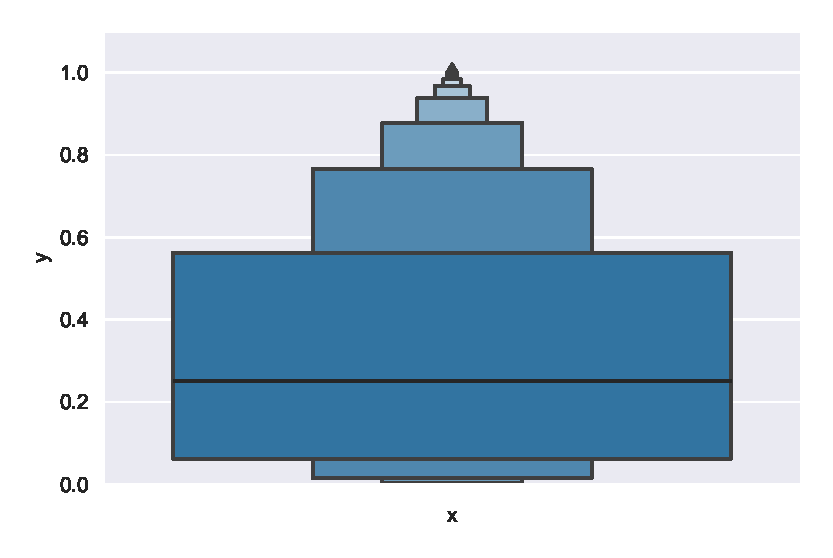
\includegraphics[scale=0.5]
    {./content/figures/expected_even_distribution_squared_error}
    \caption{Expected squared error distribution given a uniform distribution
    of estimates.}
    \label{fig:expected_even_distribution_squared_error}
\end{figure}

\begin{figure}[htbp]
    \centering
    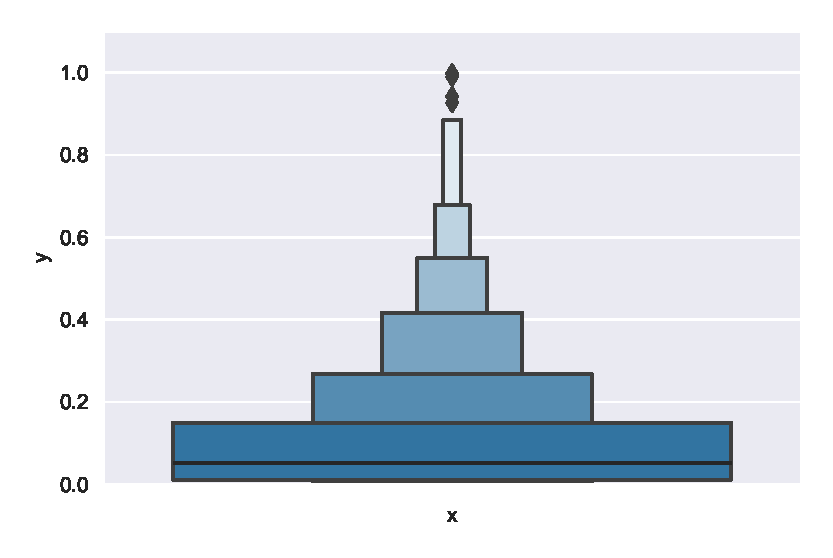
\includegraphics[scale=0.5]
    {./content/figures/expected_gaussian_distribution_squared_error}
    \caption{Expected squared error distribution given a gaussian distribution
    of estimates.}
    \label{fig:expected_gaussian_distribution_squared_error}
\end{figure}
 TODO Update

\end{document}
